\section{Released code and the configuration we reproduce}
\label{app:upstream}

\paragraph{Source.} \url{https://github.com/zhangzihan-is-good/Chisco}, commit
\texttt{e051c5b}. The README's section ``Reproducing the Paper Results'' gives:
{\small
\begin{verbatim}
python -u EEGclassify.py --rand_guess 0 --lr1 5e-4 --epoch 100 --layer 1
  --pooling mean --dataset imagine_decode --sub "01" --cls 39 --dropout1 0.5
  --dropout2 0.5 --feel1 20 --feel2 10 --subset_ratio 1
\end{verbatim}
}
Unlisted arguments take the script's defaults: batch 16, weight decay 0.01, warm-up ratio 0.1,
\texttt{--tau 0} (no logit adjustment), evaluation every 100 steps, seed 42.

\paragraph{Lines that define the protocol} (\texttt{EEGclassify.py}).
Line 74 assigns trial \texttt{index} to the evaluation set when \texttt{index \% 5 == 1};
lines 173--174 build only a training and an evaluation set; line 219 initialises \texttt{max\_accuracy} and line 263 updates it as
\texttt{max(max\_accuracy, valid\_accu)} at every evaluation; line 271 prints it as the result. The \texttt{--rand\_guess 1} option shuffles the training inputs against their labels
and leaves the evaluation set intact.

\paragraph{Running the released script.} To check our re-implementation, we also run
\texttt{EEGclassify.py} itself with the command above (seed 42) on the same hardware, with two
changes, both recorded in \path{logs/upstream_patch.diff}: the device line (\texttt{cuda}/\texttt{cpu}
$\rightarrow$ \texttt{mps}), and the two temporal convolutions replaced by the equivalent
implementation described in Section~\ref{sec:setting}. One PyTorch operator used by the
Transformer's padding-mask fast path has no MPS kernel and runs on CPU through PyTorch's
fallback setting (\path{PYTORCH_ENABLE_MPS_FALLBACK=1}). The mask is all ones, so this does not
change the computation.

\begin{figure}[h]
  \centering
  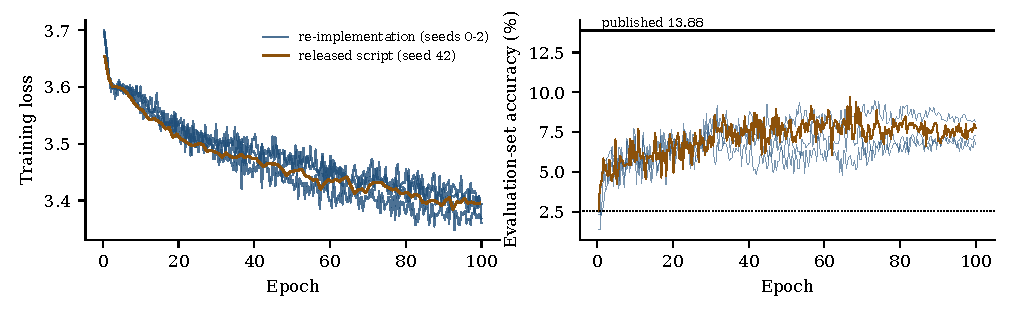
\includegraphics[width=\linewidth]{figures/fig_upstream_check.pdf}
  \caption{\textbf{Re-implementation vs.\ released script}, same configuration (500\,Hz, 100 epochs,
  released split). Left: training loss (ours: mean over each 100-step evaluation interval; released
  script: mean of its printed 10-step losses per epoch). Right: evaluation-set accuracy at every
  evaluation. Ours: seeds 0--2, trained on 4{,}495 trials; released script: seed 42, trained on
  4{,}994. Source: \texttt{results/upstream\_seed42.json} and the 500\,Hz result files.}
  \label{fig:upstream}
\end{figure}

\section{Hyperparameters and compute}
\label{app:hparams}

\begin{table}[ht]
\centering
\small
\begin{tabular}{p{0.24\linewidth}p{0.33\linewidth}p{0.33\linewidth}}
\toprule
 & Reproduction (Table~\ref{tab:repro}) & Split comparison (Table~\ref{tab:splits}) \\
\midrule
Sampling rate & 500\,Hz (1{,}651 samples) & 250\,Hz (825 samples, pairwise mean) \\
Channels & 122 EEG & 122 EEG \\
Epochs & 100 & 30 \\
Optimiser & AdamW, lr $5\times10^{-4}$, wd 0.01 & same \\
Batch size & 16 & 16 \\
Schedule & linear warm-up 10\%, then linear decay & same \\
Evaluation interval & every 100 steps (281 evaluations) & every 100 steps \\
Front end & EEGNet, $F_1{=}8$, $D{=}8$, temporal kernels 20 and 10 & same \\
Encoder & 1 Transformer layer, $d{=}64$, 8 heads, mean pooling & same \\
Dropout & 0.5 (front end), 0.5 (encoder) & same \\
Seeds & 0, 1, 2 & 0, 1, 2 \\
Folds per seed & 1 & interleaved, random: 1; run, session: 3 \\
\bottomrule
\end{tabular}
\caption{Hyperparameters of the two EEG configurations.}
\label{tab:hparams}
\end{table}

All EEG models were trained on one Apple-silicon laptop (PyTorch 2.14.1, MPS backend, float32),
three to four runs sharing the GPU. A 100-epoch run at 500\,Hz took about two hours of training time
under that sharing; the full grid of 39 configurations took about 12 hours, and the released script's
100-epoch run about three hours of training time. The no-EEG classifiers and the drift probe run on CPU in seconds to minutes.

\section{Data checks}
\label{app:data}

\begin{itemize}
\item S1 released imagined-speech epochs: 6{,}243 trials in 45 runs (28--185 per run); every
sentence maps to a category; 39 categories present.
\item In every run, the released sentences are an in-order subsequence of that run's stimulus list
(\path{textdataset/split_data_N.xlsx}); 438 of 6{,}681 presented trials are absent.
\item The BIDS release assigns S1's 45 runs to five sessions of 7, 8, 10, 10 and 10 runs. The paper
describes nine blocks per day; we use the released session labels.
\item Category composition differs between sessions: the total-variation distance between one
session's category distribution and the other four's is 0.39 for session 1 and 0.16--0.23 for the
rest. Session holdout therefore combines a leak-free split with label shift.
\end{itemize}

\section{Reproducing every number}
\label{app:repro}

All code, tests and result files accompany this paper. \texttt{scripts/fetch.sh} downloads
the public data; \texttt{scripts/reproduce\_main\_results.sh} rebuilds the cache, runs the unit
tests, the no-EEG classifiers, the drift probe, every EEG configuration, the released script, and
regenerates all tables and figures from \texttt{results/}. \texttt{paper/README.md} maps each table
and figure to the script and result file that produce it.
